\section*{\textbf{Empirical Comparison}}

We utilize a cross-sectional network measuring whether an actor indicated that they collaborated with each other during the policy design of the Swiss CO$_{2}$ act (\citealt{ingold:2008}). This is a directed relational matrix as an actor $i$ can indicate that they collaborated with $j$ but $j$ may not have stated that they collaborated with $i$. The Swiss government proposed this act in 1995 with the goal of undertaking a 10\% reduction in CO$_{2}$ emissions by 2012. The act was accepted in the Swiss Parliament in 2000 and implemented in 2008. \citet{ingold:2008}, and subsequent work by \citet{ingold:fischer:2014}, sought to determine what drives collaboration among actors trying to affect climate change policy. The set of actors included in this network are those that were identified by experts as holding an important position in Swiss climate policy. In total, Ingold identifies 34 relevant actors: five state actors, eleven industry and business representatives, seven environmental NGOs and civil society organizations, five political parties, and six scientific institutions and consultants. We follow Ingold \& Fischer and \citet{cranmer:etal:2016} in developing a model specification to understand and predict link formation in this network.\footnote{We do not review the specification in detail here, instead we just provide a summary of the variables to be included and the theoretical expectations of their effects in the Appendix.}

The LSM we fit on this network includes a two-dimensional Euclidean distance metric. The ERGM specification for this network includes the same exogenous variables as LSM, but also includes a number of endogenous characteristics of the network. The AME model we fit includes the same exogenous covariates and accounts for nodal and dyadic heterogeneity using the SRM.\footnote{Convergence diagnostics for AME are provided in the Appendix.} Third-order effects are represented by the latent factor model with $K=2$. Parameter estimates for these three approaches are shown in Table~\ref{tab:regTable}.

The first point to note is that, in general, the parameter estimates returned by the AME while similar to those of ERGM are quite different from the LSM. For example, while the LSM returns a result for the \texttt{Opposition/alliance} variable that diverges from ERGM, the AME returns a result that is similar to Ingold \& Fischer. Similar discrepancies appear for other parameters such as \texttt{Influence attribution} and \texttt{Alter's influence degree}. Each of these discrepancies are eliminated when using AME. As described previously, this is because the LSM approach complicates the interpretation of the effects of exogenous variables due to the construction of the latent variable term.\footnote{In the Appendix, we show that these differences persist even when incorporating sender and receiver random effects into the LSM.}

% latex table generated in R 3.3.1 by xtable 1.8-2 package
% Sun Aug 21 03:32:43 2016
\begin{table}[ht]
\centering
\caption{ERGM results are shown with standard errors in parentheses. LSM and AME are shown with 95\% posterior credible intervals provided in brackets.}
\begin{tabular}{lccc}
  & LSM & ERGM & AME \\
  \hline
\hline
Intercept/Edges & 0.94 & -12.17 & -3.39 \\
   & [0.09; 1.82] & (1.40) & [-4.38; -2.50] \\
  \textbf{Conflicting policy preferences}  &  &  &  \\
  $\;\;\;\;$ Business vs. NGO & -1.37 & -1.11 & -1.37 \\
   & [-2.42; -0.41] & (0.51) & [-2.44; -0.47] \\
  $\;\;\;\;$ Opposition/alliance  & 0.00 & 1.22 & 1.08 \\
   & [-0.40; 0.39] & (0.20) & [0.72; 1.47] \\
  $\;\;\;\;$ Preference dissimilarity & -1.76 & -0.44 & -0.79 \\
   & [-2.62; -0.90] & (0.39) & [-1.55; -0.08] \\
  \textbf{Transaction costs}  &  &  &  \\
  $\;\;\;\;$ Joint forum participation & 1.51 & 0.90 & 0.92 \\
   & [0.86; 2.17] & (0.28) & [0.40; 1.47] \\
  \textbf{Influence}  &  &  &  \\
  $\;\;\;\;$ Influence attribution & 0.08 & 1.00 & 1.09 \\
   & [-0.40; 0.55] & (0.21) & [0.69; 1.53] \\
  $\;\;\;\;$ Alter's influence indegree & 0.01 & 0.21 & 0.11 \\
   & [-0.03; 0.04] & (0.04) & [0.07; 0.15] \\
  $\;\;\;\;$ Influence absolute diff. & 0.04 & -0.05 & -0.07 \\
   & [-0.01; 0.09] & (0.01) & [-0.11; -0.03] \\
  $\;\;\;\;$ Alter = Government actor & -0.46 & 1.04 & 0.55 \\
   & [-1.08; 0.14] & (0.34) & [-0.07; 1.15] \\
  \textbf{Functional requirements}  &  &  &  \\
  $\;\;\;\;$ Ego = Environmental NGO & -0.60 & 0.79 & 0.67 \\
  & [-1.32; 0.09] & (0.17) & [-0.38; 1.71] \\
  $\;\;\;\;$ Same actor type & 1.17 & 0.99 & 1.04 \\
   & [0.63; 1.71] & (0.23) & [0.63; 1.50] \\
  \textbf{Endogenous dependencies}  &  &  &  \\
  $\;\;\;\;$ Mutuality &  & 0.81 & 0.39 \\
   &  & (0.25) & [-0.12; 0.96] \\
  $\;\;\;\;$ Outdegree popularity  &  & 0.95 &  \\
   &  & (0.09) &  \\
  $\;\;\;\;$ Twopaths  &  & -0.04 &  \\
  &  & (0.02) &  \\
  $\;\;\;\;$ GWIdegree (2.0)  &  & 3.42 &  \\
   &  & (1.47) &  \\
  $\;\;\;\;$ GWESP (1.0)  &  & 0.58 &  \\
   &  & (0.16) &  \\
  $\;\;\;\;$ GWOdegree (0.5)  &  & 8.42 &  \\
   &  & (2.11) &  \\
   \hline
\hline
\end{tabular}
\label{tab:regTable}
\end{table}
\FloatBarrier

There are also a few differences between the parameter estimates that result from the ERGM and AME. Using the AME we find evidence that \texttt{Preference dissimilarity} is associated with a reduced probability of collaboration between a pair of actors, which is in line with the theoretical expectations of Ingold \& Fischer.\footnote{See the Appendix for details.} Additionally, the AME results differ from ERGM for the nodal effects related to whether a receiver of a collaboration is a government actor, \texttt{Alter=Government actor}, and whether the sender is an environmental NGO, \texttt{Ego=Environmental NGO}.

\subsection*{Tie Formation Prediction}

Next, we utilize a cross-validation procedure to assess the out-of-sample performance for each of the models presented in Table~\ref{tab:regTable} as follows:

\begin{itemize}
	\item Randomly divide the $n \times (n-1)$ data points into $S$ sets of roughly equal size, letting $s_{ij}$ be the set to which pair $\{ij\}$ is assigned.
	\item For each $s \in \{1, \ldots, S\}$:
	\begin{itemize}
		\item Obtain estimates of the model parameters conditional on $\{y_{ij} : s_{ij} \neq s\}$, the data on pairs not in set $s$.
		\item For pairs $\{kl\}$ in set $s$, let $\hat y_{kl} = E[y_{kl} | \{y_{ij} : s_{ij} \neq s\}]$, the predicted value of $y_{kl}$ obtained using data not in set $s$.
	\end{itemize}
\end{itemize}

The procedure summarized in the steps above generates a sociomatrix of out-of-sample predictions of the observed data. Each entry $\hat y_{ij}$ is a predicted value obtained from using a subset of the data that does not include $y_{ij}$. In this application we set $S$ to 45 which corresponds to randomly excluding approximately 2\% of the data from the estimation.\footnote{Such a low number of observations were excluded in every sample (denoted a fold) because excluding any more observations would cause the ERGM specification to result in a degenerate model that empirically can not be fit. This is an example of the computational difficulties associated with ERGMs.} Using the set of out-of-sample predictions we generate from the cross-validation procedure, we provide a series of tests to assess model fit. The left-most plot in Figure~\ref{fig:roc} compares the five approaches in terms of their ability to predict the out-of-sample occurrence of collaboration based on Receiver Operating Characteristic (ROC) curves. ROC curves provide a comparison of the trade-off between the True Positive Rate (TPR), sensitivity, False Positive Rate (FPR), 1-specificity, for each model. Models that have a better fit according to this test should have curves that follow the left-hand border and then the top border of the ROC space. On this diagnostic, the AME model performs best closely followed by ERGM. The LSM approach lags notably behind the other specifications. 

A more intuitive visualization of the differences between these modeling approaches can be gleaned through examining the separation plots included on the right-bottom edge of the ROC plot. This visualization tool plots each of the observations, in this case actor pairs, in the dataset according to their predicted value from left (low values) to right (high values). Models with a good fit should have all network links, here these are colored by the modeling approach, towards the right of the plot. Using this type of visualization emphasizes that the AME and ERGM models perform better than the latent space approach.

\begin{figure}[ht]
	\centering
	\caption{Assessments of out-of-sample predictive performance using ROC curves, separation plots, and PR curves. AUC statistics are also provided.}
	\begin{tabular}{cc}
	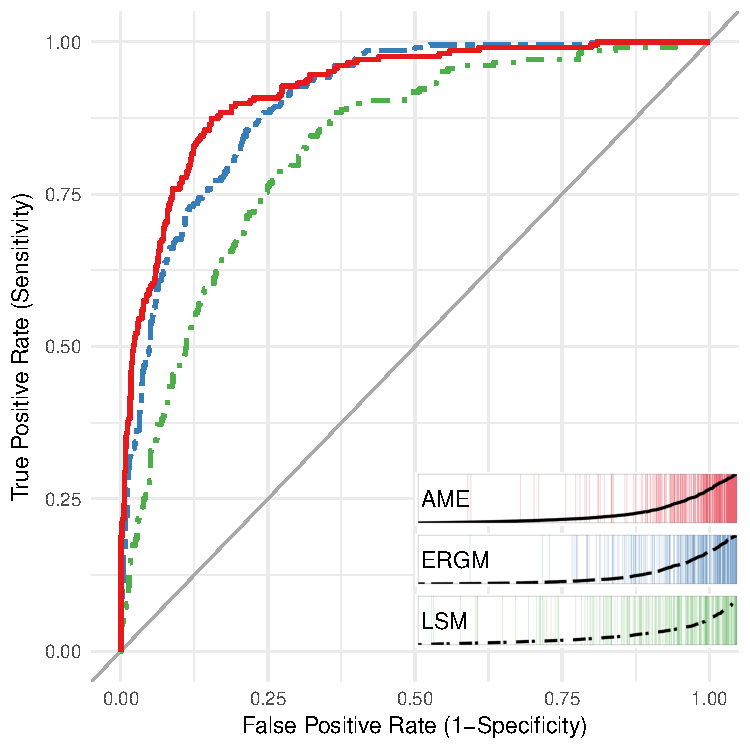
\includegraphics[width=.5\textwidth]{roc_outSampleSmall} & 
	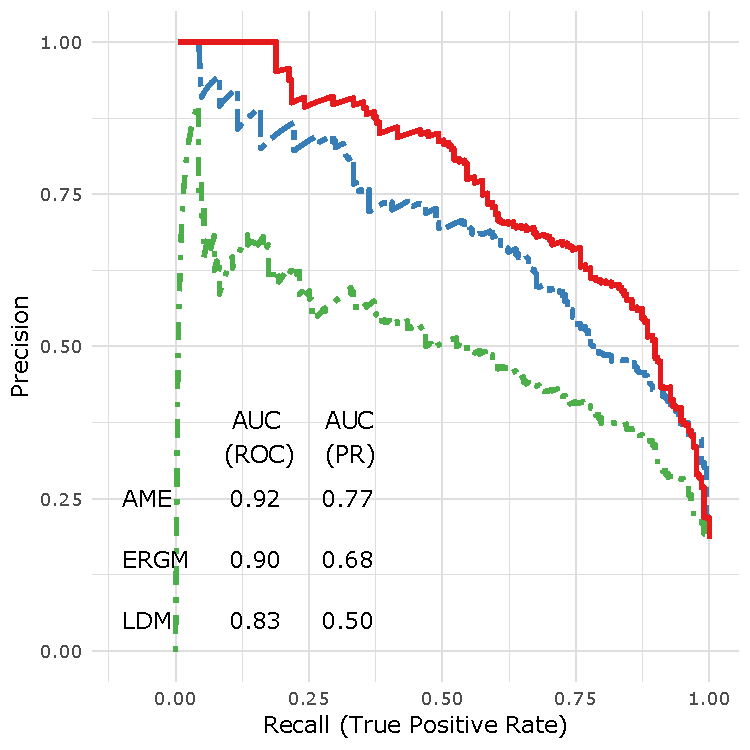
\includegraphics[width=.5\textwidth]{rocPr_outSampleSmall}	
	\end{tabular}
	\label{fig:roc}
\end{figure}

The last diagnostic we highlight to assess predictive performance are precision-recall (PR) curves. In both ROC and PR space we utilize the TPR, also referred to as recall--though in the former it is plotted on the y-axis and the latter the x-axis. The difference, however, is that in ROC space we utilize the FPR, while in PR space we use precision. FPR measures the fraction of negative examples that are misclassified as positive, while precision measures the fraction of examples classified as positive that are truly positive. PR curves are useful in situations where correctly predicting events is more interesting than simply predicting non-events (\citealt{davis:goadrich:2006}). This is especially relevant in the context of studying many relational datasets in political science such as conflict, because events in such data are extremely sparse and it is relatively easy to correctly predict non-events. In the case of our application dataset, the vast majority of dyads, 80\%, do not have a network linkage, which points to the relevance of assessing performance using the PR curves as we do in the right-most plot of Figure~\ref{fig:roc}. We can see that the relative-ordering of the models remains similar but the differences in how well they perform become much more stark. Here we find that the AME approach performs notably better in actually predicting network linkages than each of the alternatives. Area under the curve (AUC) statistics are provided in Figure~\ref{fig:roc} and these also highlight AME's superior out-of-sample performance.\footnote{We also test AME against a simple logit model and the multiple regression quadratic assignment procedure (MRQAP). Both these approaches perform worse than AME in terms of predicting tie formation. Results are available upon request.}

\FloatBarrier

\subsection*{Capturing Network Attributes}

We also assess which of these models best captures the network features of the dependent variable. To do this, we compare the observed network with a set of networks simulated from the estimated models.\footnote{In the Appendix, we compare the ability of these models to capture network attribute across a wider array of statistics (e.g., dyad-wise shared partners, incoming k-star, etc.), and the results are consistent with what we present below.} We simulate 1,000 networks from the three models and compare how well they align with the observed network in terms of four network statistics: (1) the empirical standard deviation of the row means (i.e., heterogeneity of nodes in terms of the ties they send); (2) the empirical standard deviation of the column means (i.e., heterogeneity of nodes in terms of the ties they receive); (3) the empirical within-dyad correlation (i.e., measure of reciprocity in the network); and (4) a normalized measure of triadic dependence. A comparison of the LSM, ERGM, and AME models among these four statistics is shown in Figure~\ref{fig:ergmAmePerf}.

\begin{figure}[ht]
	\centering
	\caption{Network goodness of fit summary using \pkg{amen}.}
	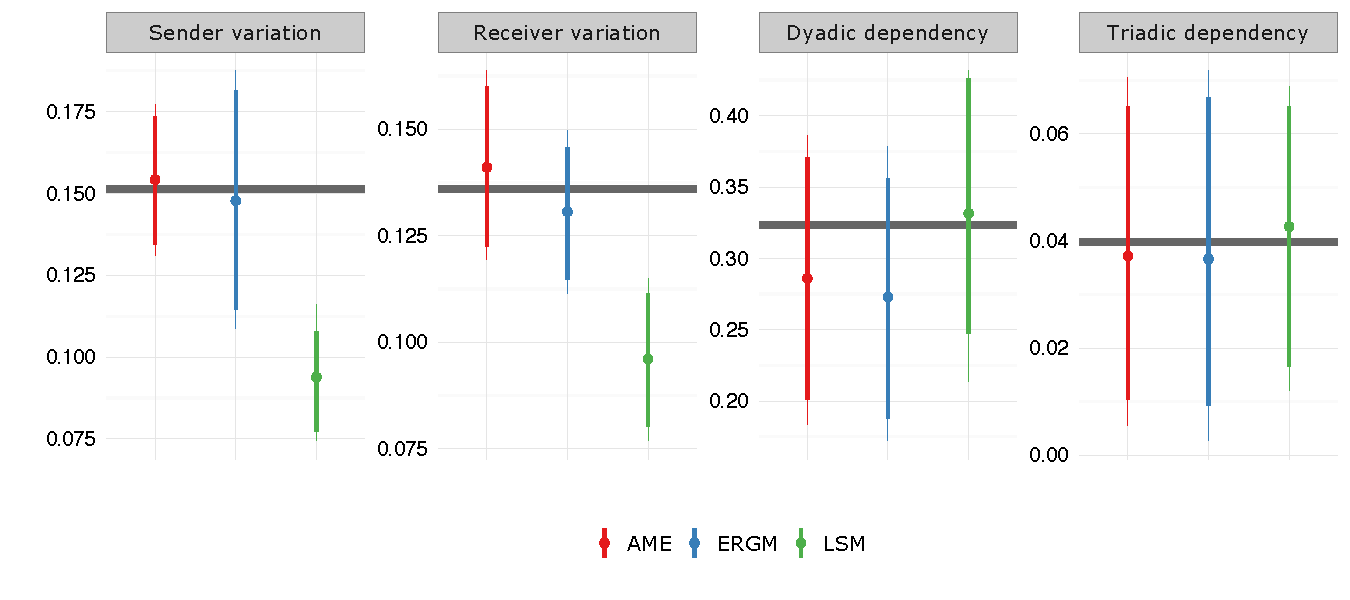
\includegraphics[width=1\textwidth]{netPerfCoef}
	\label{fig:ergmAmePerf}
\end{figure}
\FloatBarrier

Here it becomes quickly apparent that the LSM model fails to capture how active and popular actors are in the Swiss climate change mitigation network.\footnote{Further even after incorporating random sender and receiver effects into the LSM framework this problem is not completely resolved, see the Appendix for details.} The AME and ERGM specifications again both tend to do equally well. If when running this diagnostic, we found that the AME model did not adequately represent the observed network this would indicate that we might want to increase $K$ to better account for network interdependencies. No changes to the model specification as described by the exogenous covariates a researcher has chosen would be necessary. If the ERGM results did not align with the diagnostic presented in Figure~\ref{fig:ergmAmePerf}, then this would indicate that an incorrect set of endogenous dependencies have been specified. 
